\chapter{Introduction}\label{introduction}

The Roa Logic AHB-Lite Multi-layer Interconnect, hereafter referred to as 'the Interconnect', is a fully parameterized high performance, low latency interconnect fabric soft IP for AHB-Lite.
It allows a virtually unlimited number of AHB-Lite bus masters and
slaves to be connected without the need for bus arbitration to be
implemented by the bus masters. Instead, slave side arbitration is
implemented for each slave port within the core.

\begin{figure}[tbh]
  \centering
  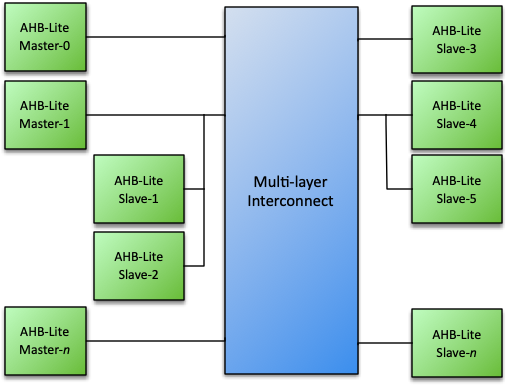
\includegraphics[scale=0.9]{assets/img/ahb-lite-switch-sys}
  \caption{Multi--layer Interconnect Usage Example}
  \label{fig:ahb-lite-switch-sys}
\end{figure}


The Multi-layer Interconnect supports priority based and round-robin based
arbitration when multiple bus masters request access to the same slave
port. Typically arbitration completes within 1 clock cycle.

\section{Features}\label{features}

\begin{itemize}
\item
  AMBA AHB-Lite compatible
\item
  Fully parameterized
\item
  Unlimited number of bus masters and slaves\footnote{The number of bus
    masters and slaves is physically limited by the timing requirements.}
\item
  Slave side arbitration
\item
  Priority and round-robin based arbitration
\item
  Slave port address decoding
\item
  Slave masking to increase system performance - New in v1.2
\item
  Error assertion when no slave correctly addressed - New in v1.3
\end{itemize}
